\chapter{Evaluation perspective on projected shifted partial derivatives}\label{chap:PSPD-more}

The measure used in the lower bounds of Kayal, Limaye, Saha, Srinivasan~\cite{KLSS} and Kumar, Saraf~\cite{KS14} was the dimension of projected shifted partials.
As seen in that chapter, the calculations are extremely delicate.
In this chapter, we shall see some slight modifications of this measure that is in a sense more \emph{algebraic} and hence useful in other lower bounds. 

\section{Coefficients vs evaluations}

For a moment, let us revisit the lower bounds of Nisan and Wigderson~\cite{nw1997}. The measure studied for the class of homogeneous depth-$3$ circuits in \autoref{thm:low-rank-sps-lb} was the dimension of partial derivatives. 
\[
\CM{NW}_k(f) \spaced{:=} \dim\set{\partial^{=k}(f)}
\]
More precisely, we interpret any element of $\partial^{=k}(f)$ as a long vector of coefficients and look at the dimension of this collection of vectors. That is, $\CM{NW}_k(f)$ is the rank of the following matrix. 

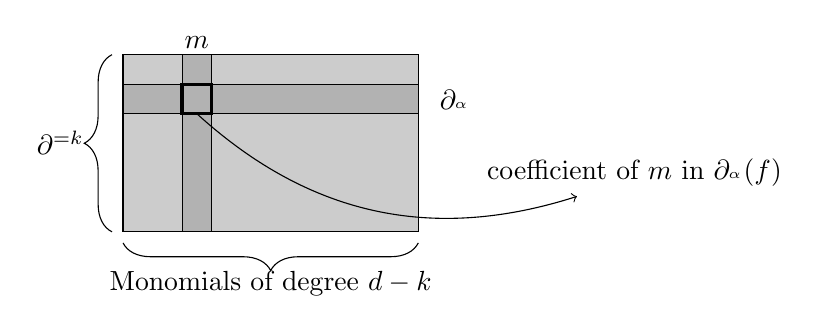
\begin{tikzpicture}[scale=0.75]
\draw[fill=black!20] (0,0) rectangle (5,3);

\draw[decorate,decoration={brace,amplitude=10pt,raise=4pt},yshift=0pt]
(0,0) -- (0,3);
\node[anchor=east] at (-0.5,1.5) {$\partial^{=k}$};
\draw[decorate,decoration={brace,amplitude=10pt,mirror, raise=4pt},yshift=0pt] 
(0,0) -- (5,0);
\node[anchor=north] at (2.5,-0.5) {Monomials of degree $d - k$};

\draw[fill=black!30] (1,0) rectangle (1.5,3);
\node at (1.25,3.2) {$m$};

\draw[fill=black!30] (0,2) rectangle (5,2.5);
\node[anchor=west] at (5.2,2.2) {$\partial_{\vecx^\alpha}$};

\draw[very thick] (1,2) rectangle (1.5,2.5);

\node[anchor=west] at (6,1) {coefficient of $m$ in $\partial_{\vecx^\alpha}(f)$}
edge[<-,bend left] (1.25,2);
\end{tikzpicture}

Grigoriev and Karpinski~\cite{grigoriev98}, for their lower bound for $\SPS$ circuits over finite fields instead looked at the dual \emph{evaluation perspective} by studying a matrix of the form

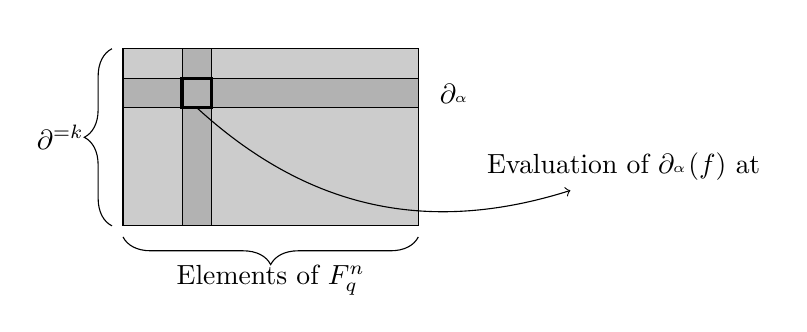
\begin{tikzpicture}[scale=0.75]
\draw[fill=black!20] (0,0) rectangle (5,3);

\draw[decorate,decoration={brace,amplitude=10pt,raise=4pt},yshift=0pt]
(0,0) -- (0,3);
\node[anchor=east] at (-0.5,1.5) {$\partial^{=k}$};
\draw[decorate,decoration={brace,amplitude=10pt,mirror, raise=4pt},yshift=0pt] 
(0,0) -- (5,0);
\node[anchor=north] at (2.5,-0.5) {Elements of $F_q^n$};

\draw[fill=black!30] (1,0) rectangle (1.5,3);
\node at (1.25,3.2) {$\veca$};

\draw[fill=black!30] (0,2) rectangle (5,2.5);
\node[anchor=west] at (5.2,2.2) {$\partial_{\vecx^\alpha}$};

\draw[very thick] (1,2) rectangle (1.5,2.5);

\node[anchor=west] at (6,1) {Evaluation of $\partial_{\vecx^\alpha}(f)$ at $\veca$}
edge[<-,bend left] (1.25,2);
\end{tikzpicture}

As seen in \autoref{chap:GK}, the measure $\CM{GK}_k$ was the rank of the above matrix (with a few columns removed).
Intuitively, we expect that if the rank of the \emph{coefficient} matrix is large, then the rank of the \emph{evaluation} matrix should also be large.
Sometimes, the evaluation perspective allows us to handle the circuit model better.
In a way, the proof of Grigoriev and Karpinski~\cite{grigoriev98} can be thought of as a formalization of this intuition for $\SPS$ circuits.
\\

A similar perspective can also be adopted for the dimension of shifted partial derivatives.
For the dimension of projected shifted partials however, this connection is not that clean.
Roughly speaking, throwing away non-multilinear monomials changes the evaluations of the shifted partials at points.
Formally, the multilinear projection of a polynomial $f$ can be interpreted as looking at the residue of $f \bmod \setdef{x_i^2}{i\in [n]}$, that is just replacing any $x_i^2$ by zero.
However this reduction does not work well with evaluations as $f(\veca)$ could be different from $(f \bmod \setdef{x_i^2}{i\in [n]})(\veca)$ for each $\veca \in \F^n$. 

Let us turn the question around and ask if we wish to understand the rank of the following matrix

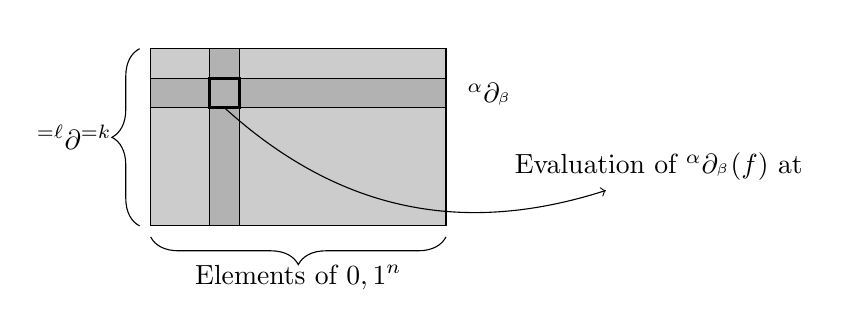
\begin{tikzpicture}[scale=0.75]
\draw[fill=black!20] (0,0) rectangle (5,3);

\draw[decorate,decoration={brace,amplitude=10pt,raise=4pt},yshift=0pt]
(0,0) -- (0,3);
\node[anchor=east] at (-0.5,1.5) {$\vecx^{=\ell}\partial^{=k}$};
\draw[decorate,decoration={brace,amplitude=10pt,mirror, raise=4pt},yshift=0pt] 
(0,0) -- (5,0);
\node[anchor=north] at (2.5,-0.5) {Elements of $\set{0,1}^n$};

\draw[fill=black!30] (1,0) rectangle (1.5,3);
\node at (1.25,3.2) {$\veca$};

\draw[fill=black!30] (0,2) rectangle (5,2.5);
\node[anchor=west] at (5.2,2.2) {$\vecx^{\alpha}\partial_{\vecx^\beta}$};

\draw[very thick] (1,2) rectangle (1.5,2.5);

\node[anchor=west] at (6,1) {Evaluation of $\vecx^\alpha\partial_{\vecx^\beta}(f)$ at $\veca$}
edge[<-,bend left] (1.25,2);
\end{tikzpicture}

\noindent
what is the \emph{coefficient} analogue of this measure?
Turns out, the answer is a different notion of projected shifted partial derivatives where the projection is not modulo $\setdef{x_i^2}{i\in [n]}$ but instead modulo $\setdef{x_i^2 - x_i}{i\in [n]}$.
It should be intuitively clear that as long as we are only interested in evaluations on $\set{0,1}^n$, the evaluation of  $f \bmod \setdef{x_i^2 - x_i}{i\in [n]}$ at $\veca\in \set{0,1}^n$ yields the same  as $f(\veca)$. 

What can we say about this modification of projected shifted partial derivatives? Is this also a measure that can give the homogeneous depth-$4$ lower bounds studied in \autoref{chap:d4hom}? Turns out the answer is indeed yes, and this perspective also allows one to generalize the lower bounds to homogeneous depth-$5$ circuits over finite fields by Kumar and Saptharishi~\cite{KumarSapt15}. There would be like the evaluation perspective of Grigoriev and Karpinski \cite{grigoriev98} (that we saw in \autoref{chap:GK}) of the lower bound of Nisan and Wigderson \cite{nw1997} (that we saw in \autoref{sec:low-rank-sps}). 

\section{Projected shifted partials via $\setdef{x_i^2-x_i}{i\in [n]}$}

The following definition is a little more general but would be useful later in this chapter. But for now, it would be useful to just consider $\mathcal{I} = \inangle{x_i^2 - x_i \;:\; i\in [n]}$. 

 \begin{definition}[PSDs with respect to $\mathcal{I}$] \label{defn:PSPD-ideal}
The \emph{projected shifted partial derivatives with respect to $\mathcal{I}$} for a polynomial $f$, denoted by $\Gamma_{k,\ell,\mathcal{I}}(f)$, is defined as 
\[
\Gamma^{\mathrm{PSD}}_{k,\ell,\mathcal{I}}(f) \spaced{:=} \dim \set{\inparen{\vecx^{=\ell} \cdot \partial^{=k}(f)} \bmod \mathcal{I}}.\qedhere
\]
\end{definition}
\noindent
In the setting where $\mathcal{I} = \inangle{x_i^2 - x_i\;:\; i\in [n]}$, every polynomial $f$, there is a unique multilinear polynomial $g$ for which $f = g \bmod \mathcal{I}$ and we shall refer to this $g$ by $f \bmod \mathcal{I}$. Thus, $\Gamma_{k,\ell,\mathcal{I}}(f)$ is the rank of the following matrix:

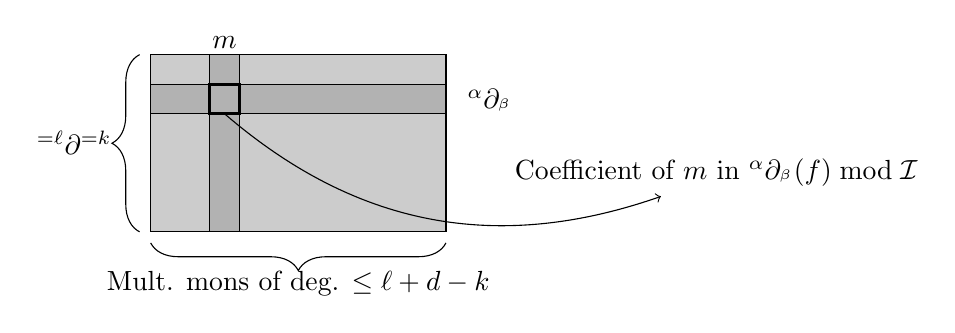
\begin{tikzpicture}[scale=0.75]
\draw[fill=black!20] (0,0) rectangle (5,3);

\draw[decorate,decoration={brace,amplitude=10pt,raise=4pt},yshift=0pt]
(0,0) -- (0,3);
\node[anchor=east] at (-0.5,1.5) {$\vecx^{=\ell}\partial^{=k}$};
\draw[decorate,decoration={brace,amplitude=10pt,mirror, raise=4pt},yshift=0pt] 
(0,0) -- (5,0);
\node[anchor=north] at (2.5,-0.5) {Mult. mons of deg. $\leq \ell + d - k$};

\draw[fill=black!30] (1,0) rectangle (1.5,3);
\node at (1.25,3.2) {$m$};

\draw[fill=black!30] (0,2) rectangle (5,2.5);
\node[anchor=west] at (5.2,2.2) {$\vecx^{\alpha}\partial_{\vecx^\beta}$};

\draw[very thick] (1,2) rectangle (1.5,2.5);

\node[anchor=west] at (6,1) {Coefficient of $m$ in $\vecx^\alpha\partial_{\vecx^\beta}(f) \bmod \mathcal{I}$}
edge[<-,bend left] (1.25,2);
\end{tikzpicture}

\noindent In \autoref{defn:PSPD}, we are essentially working with
$\mathcal{I} = \inangle{x_i^2 \;:\; i\in [n]}$ but working modulo other ideals is at times more useful.
In fact, there is a fairly large class of ideals $\mathcal{I}$ for which $f \bmod \mathcal{I}$ has a unique multilinear representative. But to make it applicable for lower bounds for homogeneous depth-$4$ circuits, we will need a mechanism to transform a ``low support polynomial'' to a ``low degree polynomial''. 

\begin{definition}[Support-to-degree ideals]\label{defn:supp-to-degree-ideal}
An ideal $\mathcal{I}$ is said to be a \emph{support-to-degree} ideal if there exist linear polynomials $\ell_1, \ldots, \ell_n$ such that
\[
\mathcal{I} \spaced{=} \inangle{x_i^2 - \ell_i(x_i) \;:\; i\in [n]}. \qedhere
\]
\end{definition}

\begin{observation}\label{obs:support-redn}
For any polynomial $f$ and a support-to-degree ideal $\mathcal{I}$, there is a unique multilinear polynomial $g$ such that $f = g \bmod\mathcal{I}$. 

Furthermore, if $f$ is a polynomial such that every monomial in $f$ depends on at most $r$ variables, then the unique multilinear polynomial $g = f \bmod\mathcal{I}$ in fact has degree at most $r$. 
\end{observation}

It is important to note that the support-to-degree ideal has generators that replace $x_i^2$ by a \emph{linear polynomial in just $x_i$}. Relaxing this to $x_i^2 - \ell$ for an arbitrary linear polynomial $\ell$ could lead to monomials of large support. 

\begin{proof}
The proof follows immediately by repeatedly replacing $x_i^2$ by $\ell_i(x_i)$.
\end{proof}

As mentioned before, we would need the above more general definition in a later lower bound but for now it would help to just keep ideals such as $\inangle{x_i^2\;:\;i\in [n]}$ or $\inangle{x_i^2 - x_i\;:\;i\in [n]}$ in mind. \\

In order to check if \autoref{defn:PSPD-ideal} is a measure useful for homogeneous depth-$4$ circuits, we need to show two things --- (1) the measure is small for a small homogeneous depth-$4$ circuit (of low bottom support), and (2) the measure is large for an explicit polynomial.
These together would imply the practicability of dimension of projected shifted partials with respect to an arbitrary support-to-degree ideal.

The second claim would be easier to prove so let us address that first. 

\begin{lemma}[PSD wrt $\mathcal{I}$ for homogeneous polynomials]\label{lem:PSD-I-lowerbound} Let $f$ be any homogeneous polynomial of degree $d$. For any choice of $k,\ell$ and any support-to-degree ideal $\mathcal{I}$, we have
\[
\Gamma^{\mathrm{PSD}}_{k,\ell,\mathcal{I}}(f) \spaced{\geq} \Gamma^{\mathrm{PSD}}_{k,\ell}(f).
\]
\end{lemma}
\begin{proof}
  Let $g \in \vecx^{=\ell} \cdot \partial^{=k}(f)$.
The main difference between $g \bmod \inangle{x_i^2\;:\; i \in [n]}$ and $g \bmod\mathcal{I}$ is just that the first projection just zeros out any non-multilinear monomial of degree $\ell + d -k$ whereas $g \bmod\mathcal{I}$ reduces non-multilinear monomials to lower degree monomials.
Hence, $g \bmod\inangle{x_i^2\;:\; i \in [n]}$ is just $g \bmod \mathcal{I}$ but just restricted to the multilinear monomials of degree $\ell + d - k$. 
Thus it follows that the rank of $\inparen{\vecx^{=\ell} \partial^{=k}g} \bmod\mathcal{I}$ is lower bounded by the rank of $\inparen{\vecx^{=\ell} \partial^{=k}g} \bmod\inangle{x_i^2\;:\; i \in [n]}$.
\end{proof}

We now want to show that if $C$ is a homogeneous depth-$4$ circuit with bottom support at most $r = O(\sqrt{d})$, then we can give a good upper bound for $\Gamma^{\mathrm{PSD}}_{k,\ell,\mathcal{I}}(C)$. 

\begin{lemma}[PSD wrt $\mathcal{I}$ for a hom. $\SPSP$ circuit]\label{lem:PSPD-I-upperbound} Let $C$ be a homogeneous $\SPSP$ computing an $n$-variate degree $d$ polynomial of top fan-in $s$ and bottom support bounded by $r$. Then for any choice of $k,\ell$ and any support-to-degree ideal $\mathcal{I}$ we have
\[
\Gamma^{\mathrm{PSD}}_{k,\ell,\mathcal{I}} \spaced{\leq} s \cdot \binom{3(d/r) + 1}{k} \cdot \binom{n}{\ell + kr}
\]
\end{lemma}
\begin{proof}
  Let us consider a single summand $T = Q_1 \cdots Q_m$ of $C$.
We shall partition this set into those polynomials $Q_1,\ldots, Q_a$ of degree at most $r$, and polynomials $Q_1',\ldots, Q_b'$ of degree more than $r$. By homogeneity of $C$, we know that $b \leq d/r$. Since some of the $Q_i$s could have very small degree, $a$ could potentially be as large as $d$. To handle this, if we find any $Q_i$ and $Q_j$ both of degree at most $r/2$, we shall replace them by their product. This ensures that all $Q_i$s have degree more than $r/2$ except perhaps one. Hence, (reusing some symbols) we can write $T$ as
\[
T \spaced{=} \tilde{Q}_1 \cdots \tilde{Q}_a \;\cdot\; Q_1' \cdots Q_b'
\]
where each $a \leq 2(d/r) + 1$, $b \leq (d/r)$, each $Q_i$ has degree at most $r$ and every monomial in a $Q_i'$ depends on at most $r$ variables. For brevity, we shall use the notation $\tilde{Q}_A$ to denote $\prod_{i\in A} \tilde{Q}_i$, and similarly $Q_B'$ to denote $\prod_{i\in B} Q_i'$. 

Let $\partial_{\vecx^\alpha}(T)$ be a $k$-th order partial derivative of $T$. By the chain rule of differentiation,
\begin{eqnarray*}
\partial_{\vecx^\alpha}(T) & \in & \mathrm{span}\setdef{ \partial_{\vecx^\beta}(\tilde{Q}_A) \cdot \partial_{\vecx^\gamma}(Q_B') \cdot \tilde{Q}_{\overline{A}} \cdot Q_{\overline{B}}'}{\begin{array}{c} \vecx^{\alpha} = \vecx^\beta \cdot \vecx^\gamma\\ |A| + |B| \leq k  \end{array}}\\
 & \subseteq & \mathrm{span}\setdef{ \vecx^{\leq k(r - 1)} \cdot \partial_{\vecx^\gamma}(Q_B') \cdot \tilde{Q}_{\overline{A}} \cdot Q_{\overline{B}}'}{\begin{array}{c} \vecx^{\alpha} = \vecx^\beta \cdot \vecx^\gamma\\ |A| + |B| \leq k  \end{array}}\\
\implies \vecx^{=\ell} \cdot \partial_{\vecx^\alpha}(T) & \subseteq & \mathrm{span}\setdef{ \vecx^{\leq \ell + k(r - 1)} \cdot \partial_{\vecx^\gamma}(Q_B') \cdot \tilde{Q}_{\overline{A}} \cdot Q_{\overline{B}}'}{\begin{array}{c} \vecx^{\alpha} = \vecx^\beta \cdot \vecx^\gamma\\ |A| + |B| \leq k  \end{array}}
\end{eqnarray*}
We now have to look at $\vecx^{=\ell} \cdot \partial_{\vecx^\alpha}(T) \bmod\mathcal{I}$ and for that notice that $Q_B'$ is a product of polynomials of low-support, that is each monomial $Q_i'$ depends on at most $\sqrt{d}$ variables. Therefore, by applying the product rule on $\partial_{\vecx^{\gamma}}(Q_B')$, we know that this can be written as a linear combination of products of low-support polynomials. By \autoref{obs:support-redn}, every polynomial $f$ of support at most $r$ there is a unique multilinear polynomial $g = f\bmod \mathcal{I}$ of degree at most $r$. Hence, we get that
\begin{eqnarray*}
\vecx^{=\ell} \cdot \partial_{\vecx^\alpha}(T) \bmod\mathcal{I} & \subseteq& \mathrm{span}\setdef{ \vecx^{\leq \ell + k(r - 1)} \cdot \vecx^{\leq k(r)} \cdot \tilde{Q}_{\overline{A}} \cdot Q_{\overline{B}}'}{\begin{array}{c} \vecx^{\alpha} = \vecx^\beta \cdot \vecx^\gamma\\ |A| + |B| \leq k  \end{array}} \bmod \mathcal{I}\\
& = & \mathrm{span}\setdef{ \vecx^{\leq \ell + kr} \cdot \tilde{Q}_{\overline{A}} \cdot Q_{\overline{B}}'}{\begin{array}{c} \vecx^{\alpha} = \vecx^\beta \cdot \vecx^\gamma\\ |A| + |B| \leq k  \end{array}} \bmod \mathcal{I}.
\end{eqnarray*}
\noindent
Therefore, an upper bound on $\set{\vecx^{=\ell} \partial^{=k}(T) \bmod \mathcal{I}}$ is 
\[
\binom{2(d/r) + 1 + (d/r)}{k} \cdot \binom{n}{\ell + kr} \cdot n
\]
\noindent
Hence, if $C = T_1 + \cdots + T_s$, then by sub-additivity we get
\[
\Gamma^{\mathrm{PSD}}_{k,\ell,\mathcal{I}}(C) \spaced{=} s \cdot \binom{3(d/r) + 1}{k} \cdot \binom{n}{\ell + kr} \cdot n.\qedhere
\]
\end{proof}

\noindent
The bound above is almost the same as in \autoref{lem:upper-bound-low-supp} and the difference is only $\exp(O(d/r))$ due to the first binomial coefficient above. \autoref{lem:PSD-I-lowerbound} and 
\autoref{lem:d4hom-goldilocks-LB} yields a lower bound for $\Gamma^{\mathrm{PSD}}_{k,\ell,\mathcal{I}}(\NW)$ as well. \\

What did we gain by looking at $\Gamma^{\mathrm{PSD}}_{k,\ell,\mathcal{I}}$ at the end of all this?
The key point is makes it easier to look at the evaluation perspective for such measures when the ideal $\mathcal{I}$ \emph{cooperates} with the evaluation operation.
A concrete instance of this was the lower bound by Kumar and Saptharishi~\cite{KumarSapt15} for homogeneous depth five circuits over finite fields.

\section{Lower bounds for depth five circuits over finite fields}

The plan would be to combine the ideas from the lower bound of Grigoriev and Karpinski \cite{grigoriev98} (discussed in \autoref{chap:GK}) with the above perspective of projected shifted partial derivatives.
The main theorem of this chapter would be the result of Kumar and Saptharishi~\cite{KumarSapt15}.

\begin{theorem}[\cite{KumarSapt15}]\label{thm:Kumar-Sapt-d5-thm}
Consider $\NW_{d,m,e}$ for some suitable choice of parameter. For any finite field $\F_q$, any homogeneous depth-$5$ circuit computing $\NW_{d,m,e}$ must be of size $\exp(\Omega_q(\sqrt{d}))$. 
\end{theorem}

\noindent 
The plan that one could adopt is the following. 
\begin{enumerate}
\itemsep 0pt
\item\label{item:PSPD-1} Take the measure to be $\Gamma^{\mathrm{PSD}}_{k,\ell,\mathcal{I}}$ where $\mathcal{I} = \inangle{x_i^q - x_i \;:\; i\in [n]}$, which is the \emph{evaluation perspective} of the shifted partial derivatives on $\F_q^n$.
\item\label{item:PSPD-2} As an analogue of ``support'' for the hom. $\SPSP$ lower bounds, we shall look at the ``rank'' of products of linear polynomials computed by the bottom two layers of the circuit. 
\item\label{item:PSPD-3} Intuitively, any term of rank at most $r$ should essentially behave like a term of degree at most $(q-1)r$, as $\mathcal{I}$ reduces any variable of exponent $q$ or above. 

Hence, the ``low-rank'' part of the circuit (only considering terms of rank at most $\sqrt{d}$) should behave like a homogeneous $\SPSP^{[q\sqrt{d}]}$ circuit, for which we can upper bound the measure in a similar fashion. 
\item\label{item:PSPD-4} To eliminate the ``high-rank'' products of linear polynomials, just as in the lower bound of Grigoriev and Karpinski \cite{grigoriev98} (as discussed in \autoref{chap:GK}), these ``high-rank'' gates are zero on almost all evaluations. 
Therefore, we can modify our measure to not look at all evaluations on $\F_q^n$ but instead at $\F_q^n \setminus \mathcal{E}$ where $\mathcal{E}$ a tiny subset of $\F_q^n$ (of about $\exp(-\sqrt{d}) \cdot q^n$ size). 

\item\label{item:PSPD-5} For the hard polynomial $\NW_{d,m,e}$, hopefully the measure continues to remain large even under the evaluation perspective on $\F_q^n \setminus \mathcal{E}$. 
\end{enumerate}

This is certainly a legitimate plan but the difficulty is in proving~\autoref{item:PSPD-5}.
The calculations for the projected shifted partials were intricate enough, and it unclear how to convert those to the evaluation perspective with a few columns removed.
Furthermore, it is important to keep the rough ballpark of parameters in mind.
If we are hoping to have parameters for $k$ and $\ell$ similar to those in \autoref{chap:d4hom}, then we are dealing with matrices with roughly $2^n \cdot \exp(O(\sqrt{d}\log n))$ rows (indexed by derivatives of order $k = O(\sqrt{d})$ and shifts of order $\ell \approx n/2$) but close to $q^n$ columns.
It would have been fine if we actually had all $q^n$ columns but we have to instead work with evaluations only on $\F_q^n \setminus \mathcal{E}$ for a set $\mathcal{E}$ of size $\exp{(-\sqrt{d})} \cdot q^n \gg 2^n$. 

In \autoref{chap:GK}, we used the property that any linear combination of determinantal minors have many non-zero evaluations. Such a statement is simply false for this setting as we are dealing with polynomials that are multiplied by monomials of degree $\approx n/2$ and are hence going to be zero at many evaluations. Therefore, one needs a different strategy. \\

{\bf Idea 1:} Since we are dealing with a matrix of evaluations, it can be naturally written as a product of a ``coefficient matrix'' and a ``Vandermonde matrix''.

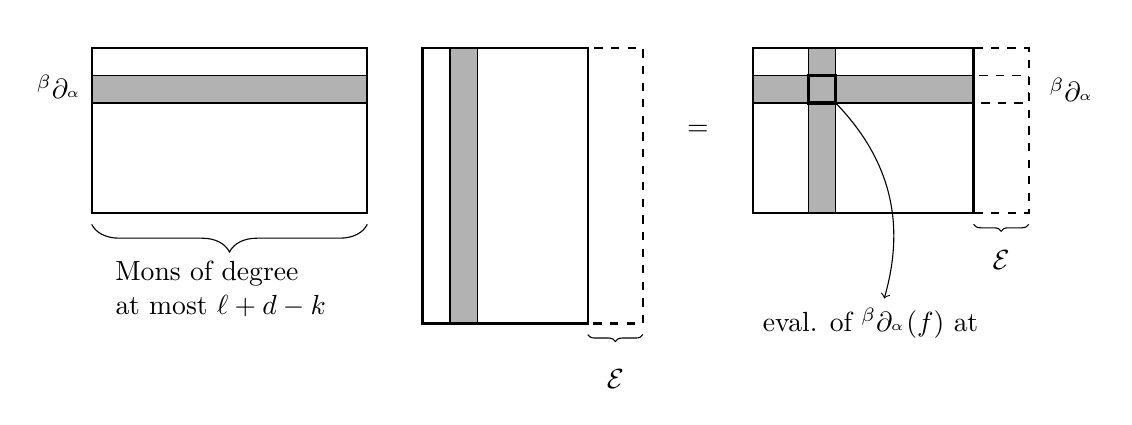
\begin{tikzpicture}[scale=0.7]
  \draw[decorate,decoration={brace,amplitude=10pt,mirror, raise=4pt},yshift=0pt] 
  (0,0) -- (5,0);
  \node[anchor=north,text width=5cm] at (4,-0.7) {Mons of degree\\at most $\ell + d - k$};
  \draw[fill=black!30] (0,2) rectangle (5,2.5);
  \draw[dashed,thick] (9,-2) rectangle (10,3);
  \draw[decorate,decoration={brace,mirror, raise=4pt},yshift=0pt] 
  (9,-2) -- (10,-2);
  \node at (9.5,-3) {$\mathcal{E}$};
  \draw[fill=black!30] (6.5,3) rectangle (7,-2);
  \node at (6.75,3.2) {$\veca$};
  \node[anchor=east] at (0,2.25) {$\vecx^{\beta}\partial_{\vecx^\alpha}$};
  \draw[thick] (6,-2) rectangle (9,3);
  \draw[thick] (0,0) rectangle (5,3);

  \begin{scope}[shift={(12,0)}]
  \node at (-1,1.5) {$=$};
  \draw[decorate,decoration={brace,mirror, raise=4pt},yshift=0pt] 
  (4,0) -- (5,0);
  \node[anchor=north] at (4.5,-0.5) {$\mathcal{E}$};
  
  \draw[fill=black!30] (1,0) rectangle (1.5,3);
  \node at (1.25,3.2) {$\veca$};
  
  \draw[fill=black!30] (0,2) rectangle (4,2.5);
  \draw[dashed] (4,2) rectangle (5,2.5);
  \node[anchor=west] at (5.2,2.2) {$\vecx^{\beta}\partial_{\vecx^\alpha}$};
  
  \draw[very thick] (1,2) rectangle (1.5,2.5);
  
  \node[anchor=west] at (0,-2) {eval. of $\vecx^{\beta}\partial_{\vecx^\alpha}(f)$ at $\veca$}
  edge[<-,bend right] (1.5,2);
  \draw[thick] (0,0) rectangle (4,3);
  \draw[dashed,thick] (4,0) rectangle (5,3);
  \end{scope}
\end{tikzpicture}

Formally, let $C$ be  a matrix with rows indexed by shifted partials and columns indexed by monomials of the right degree, so that each row of $C$ is just the coefficients of a shifted partial $\vecx^{\beta} \partial_{\vecx^\alpha}(f) \bmod \mathcal{I}$ listed down. Also, let $V$ be the evaluation matrix of the monomials where rows are indexed by monomials and columns indexed by points in $\F_q^n$. Then the product $C \cdot V$ is precisely the evaluation matrix of shifted partials modulo $\mathcal{I}$. Furthermore, discarding a set $\mathcal{E}$ of evaluations is just discarding the corresponding columns from $V$. 

In \autoref{chap:d4hom}, we essentially showed that the matrix $C$ for $\NW_{d,m,e}$ has pretty large row-rank.
Furthermore, it is easy to show that $V$ also has full-rank.
Since $\mathcal{E}$ is a fairly small set, we should expect $\tilde{V}$, which is $V$ with the columns indexed by $\mathcal{E}$ removed, to also have very large rank.
Can we therefore claim that $C \cdot \tilde{V}$ also has large rank?
In some sense, we  certainly can.

\begin{lemma}[Rank of products]\label{lem:rank-of-products}
For matrices $X \cdot Y = Z$, we always have that
\[
\rank(X) \spaced{\geq} \rank(Y) \;+\; \rank(Z) \;-\; (\mathrm{common\ dimension})
\]
where $\mathrm{common\ dimension}$ denotes the number of columns of $X$ or the number of rows of $Y$. 
\end{lemma}

Of course, if $\tilde{V}$ has full-rank then $\rank(M) = \rank(C)$.
The problem is that if we are forced to look at a subset of evaluations and hence $\tilde{V}$ may not be full rank.
When we are looking at all evaluations on $\F_q^n$, then the matrix $V$ and $\tilde{V}$ has much more $2^n$ rows as row indices would also involve non-multilinear monomials.
However $C$ just has $2^n$ rows and hence they could potentially all be in the left-kernel of $\tilde{V}$ thus making $C \cdot \tilde{V} = 0$.
Thus, we need a way of reducing the number of rows in $V$ to about $2^n$.
\\

{\bf Idea 2:} Do not consider evaluations on $\F_q^n$ but just evaluations on $\set{0,1}^n \subset \F_q^n$. \\

\noindent
That way, it is equivalent to reducing all polynomials $\mathcal{I} = \inangle{x_i^2 - x_i \;:\;i\in [n]}$ and hence the rows of $V$ (or columns of $C$) would be indexed by only multilinear monomials of degree at most $\ell+d-k$, which is the same regime as in \autoref{chap:d4hom}.
Hence, we can hope to use \autoref{lem:rank-of-products} to lower bound the measure for $\NW_{d,m,e}$.

The problem now becomes \autoref{item:PSPD-4}, the ``high rank'' gates.
Consider the high-rank term $(x_1 + 2) \cdots (x_n + 2)$ over say $\F_7$.
This term remains non-zero when we evaluate on any point in $\set{0,1}^n$.\\

{\bf Idea 3:} Do not consider evaluations on $\set{0,1}^n$ but rather on a \emph{shift} of $\set{0,1}^n$. \\

Picking a random point $\F_q^n$ can be thought of as first picking a point $\vecc \in \F_q^n$, and then picking a shift $\vecx \in \set{0,1}^n$ and returning $\vecc + \vecx$.
Therefore, if we have an event that is \emph{good} for a random point in $\F_q^n$, this also shows that there exists a $\vecc \in \F_q^n$ for which the event is \emph{good} for a random point in $\vecc + \set{0,1}^n$.

\begin{lemma}\label{lem:shift-of-hypercube-averaging}
Let $A$ be an function on $\F_q^n$ and suppose $\E_{\vecy \in \F_q^n}[A(\vecy)] \geq \delta$. Then, there exists a point $\vecc \in \F_q^n$ such that 
\[
\E\limits_{\vecy \in \vecc + \set{0,1}^n}[A(\vecy)] \spaced{\geq} \delta
\]
\end{lemma}

In this setting, if the event is the vanishing of all high-rank gates, we now have that there exists a \emph{translate of a hypercube} $\vecc + \set{0,1}^n$ such all high rank gates vanish on most points in this translate of a hypercube.

We are now back to~\autoref{item:PSPD-5}, lower bounding the rank of the evaluation matrix for $\NW_{d,m,e}$.
Since we are only dealing with a translate of a hypercube, we can finding a support-to-degree ideal $\mathcal{I}$ that respects evaluations on $\vecc + \set{0,1}^n$.

\begin{lemma}[\cite{KumarSapt15} Multilinearization for translate of hypercubes]\label{lem:multilinearization-translate}
  Let $\vecc + \set{0,1}^n$.
Then there exists a support-to-degree ideal $\mathcal{I}$ such that every polynomial $f(\vecx) \in \F_q^n$ has a unique multilinear representative $g$ with $\deg(g) \leq \deg(f)$ that agrees with $f$ on $\vecc + \set{0,1}^n$.
\end{lemma}
\begin{proof}
  Since each $x_i$ can only take values $c_i$ or $c_i + 1$, it suffices to replace each $x_i^2$ by either $c_i^2$ or $(c_i + 1)^2$ depending on the value of $x_i$.
It is easy to find a linear polynomial $\ell_i$ such that $\ell_i(c_i) = c_i^2$ and $\ell_i(c_i+1) = (c_i+1)^2$ --- a simple calculation yields $\ell_i(x) = c_i^2 + (x - c_i)(2c_i + 1)$.
Hence, if we define $\mathcal{I}$ to be
\[
\mathcal{I} \spaced{=} \setdef{x_i^2 - c_i^2 - (x_i - c_i)(2c_i + 1)}{i\in [n]},
\]
clearly this is a support-to-degree ideal (\autoref{defn:supp-to-degree-ideal}) and by definition does not alter the evaluation on $\vecc + \set{0,1}^n$. 
\end{proof}

With this multilinearization lemma, the coefficient matrix $C$ has columns indexed by just multilinear monomials of degree at most $\ell + d - k$ which makes the dimensions $C$ more balanced. 

These are the main ideas that go into the proof of Kumar and Saptharishi \cite{KumarSapt15} and from here on is just setting the right parameters etc.
The rest of the exposition will leave a lot of the proofs as exercises to the readers as the main intuitions have been exposed.

\subsubsection*{The formal measure}

For a set $\mathcal{A} \subseteq \F_q^n$, define the measure $\CM{KS}_{k,\ell,\mathcal{A}}$ as follows
\[
\CM{KS}_{k,\ell,\mathcal{A}}(f) \spaced{=} \rank \set{\inparen{\vecx^{= \ell} \cdot \partial^{=k}(f)  }_{\veca \in \mathcal{A}}}
\]
or in other words is the rank of the matrix where rows are indexed by shifts and partial derivatives, columns are indexed by elements $\mathcal{A}$ and the corresponding entry being the evaluation of the shifted partial derivative of $f$ at the point $\veca$.

\subsection{Upper bound for a homogeneous depth-$5$ circuit}

The upper bound would proceed in the following natural steps, similar to the discussion in \ref{chap:GK}. 

\begin{lemma}[\cite{KumarSapt15} Eliminating high-rank gates]
  Let $C$ be a homogeneous depth-$5$ circuit that computes an $n$-variate degree $d$ polynomial over $\F_q$.
Assume that $\mathrm{size}(C) \leq 2^{\sqrt{d}/100}$.
Let $\tau = q\sqrt{d}/6$ and $k = \tau / 2q^3 = O_q(\sqrt{d})$.
Then, there is a set $\mathcal{E}$ of size at most $\exp{-O(\sqrt{d})} \cdot q^n$ such that all products of linear polynomials of rank greater than $\tau$ that are computed by the bottom to layers of $C$ vanish on all of $\F_q^n \setminus \mathcal{E}$ with multiplicity at least $k$.
\end{lemma}
\begin{exercise}
Prove this. 
\end{exercise}


\begin{lemma}[\cite{KumarSapt15} Upper bound]\label{lem:PSPD-more-upper-bound-ckt}
Let $C$ be a homogeneous depth-$5$ circuit of size at most $2^{\sqrt{d}/100}$ that computes an $n$-variate degree $d$ polynomial over $\F_q$. Let $\tau, k, \mathcal{E}$ be as above. 
Then, for any $\mathcal{A} \subset \F_q^n \setminus \mathcal{E}$ that is contained in some $\vecc + \set{0,1}^n$, we have
\[
\CM{KS}_{k,\ell,\mathcal{A}}(C) \spaced{\leq} 2^{\sqrt{d}/100} \cdot \binom{\frac{4d}{\tau} + 1}{k} \cdot \binom{n}{\ell + k\tau q} \cdot \poly(n)
\]
\end{lemma}

This proof would proceed in a few steps. 

\begin{claim}
Consider the polynomial $C'$ which is obtained from $C$ by \emph{dropping all products of linear polynomials or rank at least $\tau$}. Then, by the choice of $\mathcal{A}$,
\[
\CM{KS}_{k,\ell,\mathcal{A}}(C) \spaced{=}\CM{KS}_{k,\ell,\mathcal{A}}(C')
\]
\end{claim}

\begin{claim}
  If $C'$ is a homogeneous depth-$5$ circuit with all products of linear forms having rank at most $\tau$, and if $\mathcal{A}$ is contained in some translate of a hypercube $\vecc + \set{0,1}^n$, then
\[
\CM{KS}_{k,\ell,\mathcal{A}}(C') \spaced{=} \mathrm{size}(C') \cdot \binom{\frac{4d}{\tau} + 1}{k} \cdot \binom{n}{\ell + k\tau q} \cdot \poly(n)
\]
\end{claim}

\begin{exercise}
Complete the proofs using \autoref{obs:support-redn} and \autoref{lem:multilinearization-translate}. 
\end{exercise}

\subsection{Lower bound for $\NW_{d,m,e}$}

As mentioned earlier, to lower bound the rank of the evaluation matrix we shall write this as $C \cdot V$ and use \autoref{lem:rank-of-products} to lower bound the rank.
The matrices $C$ and $V$ shall be the following:
\begin{quote}
{\bf The matrix $C$:}

Rows are indexed by shifted partials, columns are indexed by multilinear monomials of degree at most $\ell + d - k$, and the entry in $(\vecx^{\alpha} \cdot \partial_{\vecx^{\beta}} , m)$ is the coefficient of the monomial $m$ in the unique multilinear representative of $\vecx^{\alpha} \cdot \partial_{\vecx^{\beta}}(f) \bmod{\mathcal{I}}$ (\autoref{lem:multilinearization-translate}). 

{\bf The matrix $V({\mathcal{A}})$:} 

Rows are indexed by multilinear monomials of degree at most $\ell + d - k$, columns are indexed by points in $\mathcal{A}$, and the entry at $(m,\veca)$ is the evaluation of $m$ at $\veca$.
\end{quote}

We shall set parameters in $\NW_{d,m,e}$ as we had in \autoref{lem:d4hom-goldilocks-LB}, then by \autoref{lem:PSD-I-lowerbound}, we have the following bound for the rank of $C$.

\begin{eqnarray}
\rank(C) & \geq & \binom{n}{\ell} \cdot (1 + \epsilon)^{2d-2k} \cdot \exp(-O(\log^2 n))\nonumber\\
 & = & \binom{n}{\ell + d - k} \cdot \exp(-O(\log^2 n))\label{eqn:rank-C-lower-bound}
\end{eqnarray}

Moving on to the rank of $V(\mathcal{A})$.
Currently, $\mathcal{A}$ is contained in some translate $\vecc + \set{0,1}^n$.
The following observation allows us to instead look at subsets of $\set{0,1}^n$, which is easier to study.

\begin{observation} For any set $\mathcal{A}$ and a point $\vecc \in \F_q^n$, we have 
\[
\rank(V(\mathcal{A}) = \rank(V(\mathcal{A} - \vecc)). 
\]
\end{observation}
\begin{exercise}
Prove this. 
\end{exercise}

Due to this observation, we might as well assume that $\mathcal{A} \subset \set{0,1}^n$.
Suppose we consider the simpler matrix $\tilde{V}$ where we have a column for every $\veca \in \set{0,1}^n$.
How do we show that $\tilde{V}$ has full rank?
This is because the matrix $\tilde{V}$ has an lower-triangular matrix sitting inside with ones on the diagonal.
To elaborate a bit, if we were to order the rows by decreasing order of degrees, and match each row (monomial) by the characteristic vector (a point $\veca$ of hamming weight at most $\ell + d - k$), then it is easy to see that this is a lower-triangular matrix with ones on the diagonal.

Due to this, if it so happens that $\mathcal{A}$ has many points from 
\[\mathcal{H}_{\leq \ell+ d - k} = \setdef{\veca \in \set{0,1}^n}{\mathrm{wt}(\veca) \leq \ell + d - k},\]
then $\rank(V)$ would also be large.
The point is that we only need to avoid the set $\mathcal{E}$ but we are free to choose any translate we want.
The same averaging argument comes into play here to ensure that we have a large intersection with a translate of $\mathcal{H}_{\leq \ell+ d - k}$.
\begin{lemma}
Let $\mathcal{E} \subset \F_q^n$ be a set of size $\delta \cdot q^n$. Then, there exists $\vecc \in \F_q^n$ such that 
\[
\abs{(\vecc + \mathcal{H}_{\leq \ell+ d - k}) \intersection \mathcal{E}} \spaced{\leq} \delta \cdot \abs{\mathcal{H}_{\ell + d - k}}
\]
\end{lemma}

From this lemma, the rank bound follows. 

\begin{lemma}
For any set $\mathcal{E} \in \F_q^n$ of size at most $\delta \cdot q^n$, there exists a set $\mathcal{A}$ that is contained in some $\vecc + \set{0,1}^n$ for which 
\[
\rank(V(\mathcal{A})) \spaced{\geq} \binom{n}{\ell + d - k} \cdot (1 - \delta)
\] 
\end{lemma}
\begin{exercise}
Prove this. 
\end{exercise}

Putting all of this together yields the require lower bound for the rank of the evaluation matrix for $\NW_{d,m,e}$. 

\begin{lemma}
Let the parameters of $\NW_{d,m,e}$ be chosen appropriately. Then, for any set $\mathcal{E} \subset \F_q^n$ of size at most $\exp(-O(\sqrt{d})) \cdot q^n$, there exists a set $\mathcal{A}$ contained in $\vecc + \set{0,1}^n$ and is disjoint from $\mathcal{E}$ such that
\[
\CM{KS}_{k,\ell,\mathcal{A}}(\NW_{d,m,e}) \spaced{\geq} \binom{n}{\ell + d - k} \cdot \exp(-O(\log^2 n))
\]
\end{lemma}

Combining this with \ref{lem:PSPD-more-upper-bound-ckt}, the main theorem (\autoref{thm:Kumar-Sapt-d5-thm}) of Kumar and Saptharishi~\cite{KumarSapt15} (almost\footnote{there is a slight technicality here that depending on $F_q$ we choose $k$ accordingly and hence we get that ``for each $q$ there is a polynomial $f$ for which the bound holds''.
This can be fixed to instead get the right order of quantifiers --- ``There is a polynomial $f$ such that for every $q$ ...''})
follows.

%%% Local Variables: 
%%% mode: latex
%%% TeX-master: "fancymain"
%%% End: 
